\chapter{Physical Setup}\label{ch:physsetup}
\section{Pumps}
\todo[color=03physicalSetup]{talk more about the pumps used, because the only reason we use them is: "they are present in the setup", e.g. we don't care why other pumps are not as good. [debatable]}
\subsection{Principle}
Centrifugal pumps are the most commonly used type of pump, due to its many advantages, simple construction, relative low 
cost, reliability and quiet operation.

When the pump is in operation, an increase in the fluid pressure from the pump's inlet to its outlet is created. This pressure 
difference drives the fluid further through the system.

The pump creates a pressure difference by transferring mechanical energy from the motor to the fluid through the impeller. The fluid 
flows from the inlet to the impeller center and out along its blades.
The centrifugal force increases the fluid velocity and consequently the kinetic energy is transformed to pressure. 

The blades of the rotating impeller transfer energy to the fluid by increasing velocity and pressure. The fluid is sucked into the 
impeller at the impeller eye and flows through the impeller channels formed by the blades between the shroud and hub.

The design of the impeller depends on the requirements for application, pressure and flow. The impeller is the primary component 
determining the pump performance. Pumps variants are often created only by modifying the impeller.
\todo[color=03physicalSetup]{maybe a bit repetitive, formatting could be improved }

Figure \ref{fig:pump_sections} represents the cross section and the transverse section of a centrifugal pump.
\newpage
\begin{figure}[h]
    \centering
    \subfloat[Cross Section]{{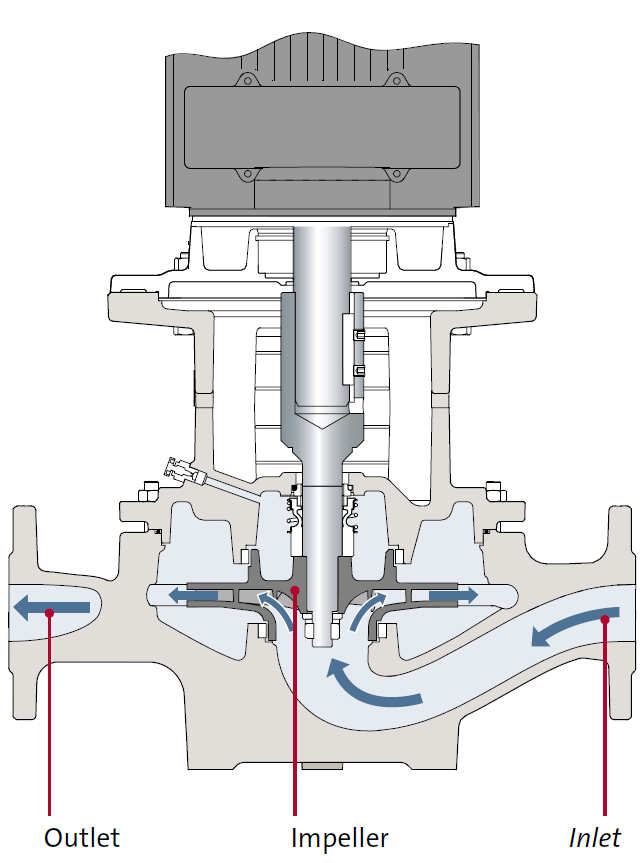
\includegraphics[width=0.4\linewidth]{figures/pump_cross_section.PNG}}}
    \qquad
    \hfill
    \subfloat[Transverse Section]{{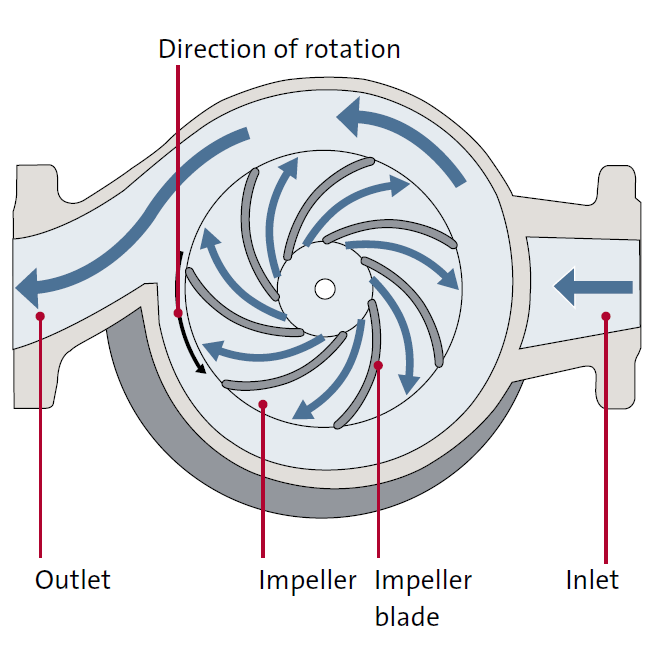
\includegraphics[width=0.4\linewidth]{figures/pump_above_view.PNG}}}
    \caption{Centrifugal Pump}
    \label{fig:pump_sections}
\end{figure}

\subsection{Affinity Laws}
Affinity laws are mathematical relationships that provide a way to estimate the changes in performance of a pump, as a result
of a change in one of the basic pump variables.
In it's simplest form, the term law, means a principle that has been proven true for all cases.
\todo[color=03physicalSetup]{add affinity laws, formula and statement}
\todo[color=03physicalSetup]{"proven true for all cases"? that can't be correct for an estimate}

\begin{equation}
	\left(\frac{N_1}{N_2}\right)^1 = \frac{Q_1}{Q_2}$$
	
	$$\left(\frac{N_1}{N_2}\right)^2 = \frac{H_1}{H_2}$$
	
	$$\left(\frac{N_1}{N_2}\right)^3 = \frac{P_1}{P_2}	
\end{equation} Equations for constant impeller diameter $D$ \cite{AffinityLaws}

\begin{equation}
	\left(\frac{D_1}{D_2}\right)^1 = \frac{Q_1}{Q_2}$$
	
	$$\left(\frac{D_1}{D_2}\right)^2 = \frac{H_1}{H_2}$$
	
	$$\left(\frac{D_1}{D_2}\right)^3 = \frac{P_1}{P_2}	
\end{equation} Equations for constant rotational speed $N$ \cite{AffinityLaws}


\subsection{Performance Curves}

\section{Pipes}
Pipes are a way of transporting liquids or gasses, inside a controllable environment.
They are used to interconnect the pumps and the tank and other peripherals.
One common analogy compares them to wires in electrical circuits.

Based on their diameters, material and shape,
they introduce resistance to the flow of the pumped medium.
Staying with the analogy to electrical circuits,
this can be compared to the cross sectional area and the specific resistance of a wire material.

\section{Valves}
Valves can control the resistance introduced, by changing the diameter of the pipeline at a given point. \todo[color=03physicalSetup]{re-write valves, this reads terrible}

The valve built into the used system is not used for control purposes,
but only to simulate disturbances downstream the pumps.

Depending on the type of valves, they can block the flow partially or completely.
Their reaction and settling time may change and their ability to withstand pressure.
Some valves have an inbuilt controller, managing the opening percentage.
Valves can be actuated by different means, for example air pressure, electric motors or handles
\todo[color=03physicalSetup]{there is a better word for handle in this context}

\section{Sensors}
To be able to monitor the system closely, different sensors are used.
\todo[color=03physicalSetup]{write about the sensors used in the system}

\subsection{Flow Meter}
\subsection{$\Delta$Pressure Sensor}
\subsection{Power Sensor}
\todo[color=03physicalSetup]{complete this list of subsections}
\todo[color=03physicalSetup]{maybe take out of ToC? (subsection*)}

\todo[color=03physicalSetup]{Do we want a section about xPC and Simulink Realtime?}
